\documentclass[12pt,a4paper]{article}

\usepackage[T1]{fontenc}
\usepackage[utf8]{inputenc}
\usepackage{lmodern}
\usepackage{amsmath,amssymb}
\usepackage{graphicx}
\usepackage{booktabs}
\usepackage[hidelinks]{hyperref}
\usepackage{geometry}
\geometry{margin=2.5cm}

\graphicspath{{figures/}{../results/}}

\title{Neural Style Transfer: \\ A Comparison of the VGG16, VGG19 and ResNet50 Backbones}
\author{Nikita S.}
\date{2022}

\begin{document}
\maketitle

\begin{abstract}
This work implements neural style transfer by image optimization~\cite{gatys2016}
and compares three pretrained convolutional networks used as feature extractors:
VGG16, VGG19~\cite{simonyan2015} and ResNet50~\cite{he2016}. We show that the
VGG family yields visually more convincing stylizations than ResNet50, and we
illustrate the method on three different content/style pairs.
\end{abstract}

\tableofcontents
\newpage

\section{Introduction}
Neural Style Transfer (NST) is the task of synthesizing an image that keeps the
\emph{content} of one photograph while adopting the \emph{artistic style} of
another. The seminal method~\cite{gatys2015, gatys2016} uses the activations of
a pretrained convolutional network as a differentiable description of content
and style, and optimizes the target image directly by gradient descent.

The goal of this work is not only to reproduce the method, but also to study how
the choice of feature-extractor architecture affects the result. To this end,
the same feature-extraction scheme is applied to three networks: VGG16, VGG19
and ResNet50.

\section{Method}

\subsection{Feature extraction}
Let $F^{l}\in\mathbb{R}^{C_l\times H_l\times W_l}$ be the activation map at layer
$l$. For VGG networks the activations are taken after each Conv${+}$ReLU pair;
for ResNet50 they are taken after each bottleneck block of all four stages. All
network weights are frozen; only the image is optimized.

\subsection{Loss functions}
\paragraph{Content.} The mean squared error between the activations of a deep
layer:
\begin{equation}
\mathcal{L}_{\text{content}} = \frac{1}{2}\sum_{i,j}\bigl(F^{l}_{ij}-P^{l}_{ij}\bigr)^{2},
\end{equation}
where $P^l$ are the activations of the content image.

\paragraph{Style.} Style is described by the Gram matrix, i.e.\ the correlations
between channels:
\begin{equation}
G^{l}_{ij} = \frac{1}{C_l H_l W_l}\sum_{k} F^{l}_{ik}F^{l}_{jk},
\qquad
\mathcal{L}_{\text{style}} = \sum_{l} w_l \,\bigl\| G^{l}-A^{l}\bigr\|_2^2,
\end{equation}
where $A^l$ is the Gram matrix of the style image. Because the Gram matrix
aggregates over all spatial positions, it captures texture and colour statistics
independently of spatial layout. The normalization by $C_l H_l W_l$ makes the
weights $w_l$ comparable across layers of different sizes.

\paragraph{Regularization.} To suppress high-frequency noise we add an isotropic
total-variation term over the \emph{spatial} axes:
\begin{equation}
\mathcal{L}_{\text{TV}} = \frac{1}{N}\sum\bigl(I_{h+1,w}-I_{h,w}\bigr)^2
                        + \frac{1}{N}\sum\bigl(I_{h,w+1}-I_{h,w}\bigr)^2 .
\end{equation}

\paragraph{Total loss.}
\begin{equation}
\mathcal{L} = \alpha\,\mathcal{L}_{\text{content}}
            + \beta\,\mathcal{L}_{\text{style}}
            + \gamma\,\mathcal{L}_{\text{TV}} .
\end{equation}

\subsection{Optimization}
The target image is initialized as a copy of the content image and optimized
with L-BFGS~\cite{liu1989lbfgs}. The constant targets (content activations and
style Gram matrices) are computed once before the optimization loop.

\section{Experiments and Results}
All three networks were run on the same content/style pair
(Fig.~\ref{fig:teaser}) at $384\times384$ resolution for 50 L-BFGS steps. The
side-by-side outputs are shown in Fig.~\ref{fig:comparison}.

\begin{figure}[htbp]
  \centering
  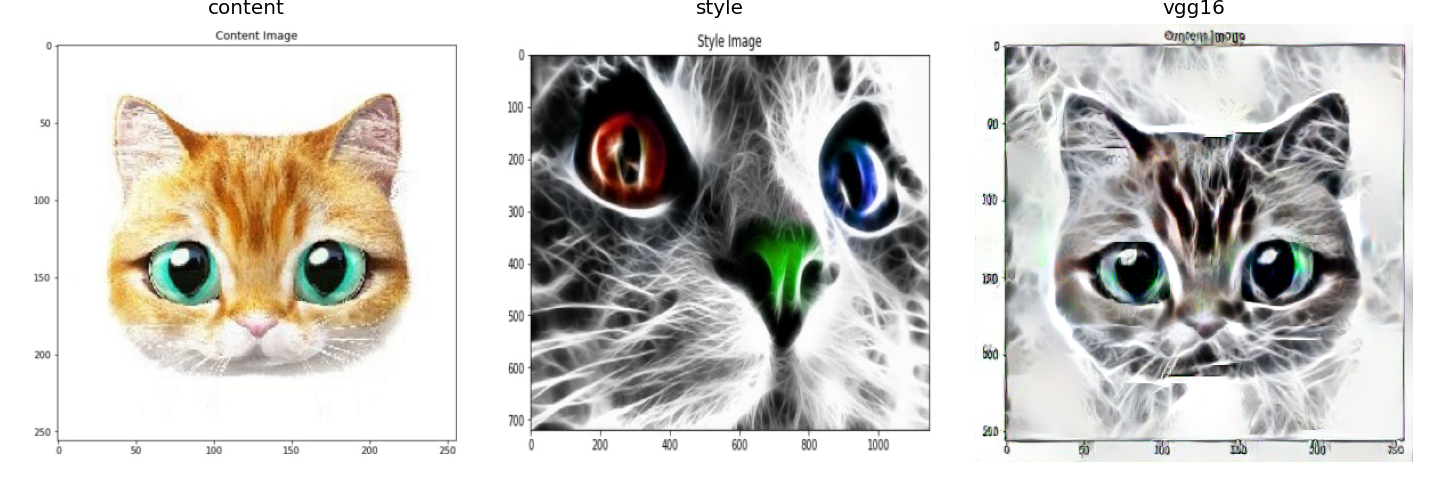
\includegraphics[width=\textwidth]{teaser.png}
  \caption{Left to right: content, style, result (VGG16).}
  \label{fig:teaser}
\end{figure}

\begin{figure}[htbp]
  \centering
  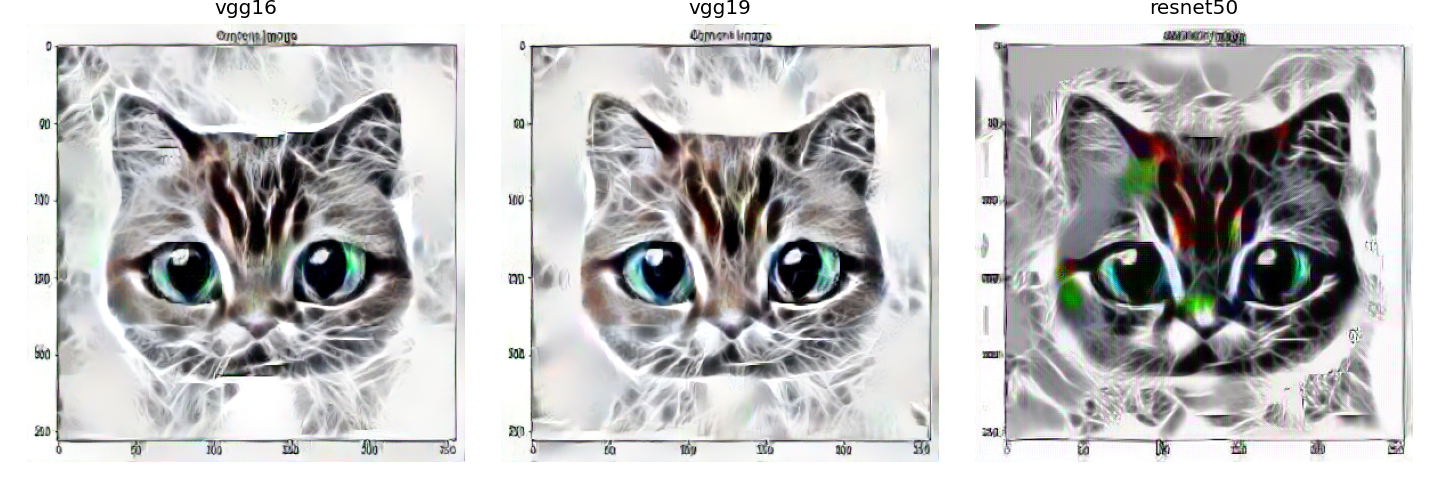
\includegraphics[width=\textwidth]{comparison.png}
  \caption{Comparison of the three architectures on the same pair.}
  \label{fig:comparison}
\end{figure}

The convergence curves in Fig.~\ref{fig:loss} show that L-BFGS reduces the total
loss monotonically for both networks; ResNet50, however, settles at a higher
residual loss, consistent with its lower visual quality. Table~\ref{tab:compare}
summarizes the qualitative comparison.

\begin{table}[htbp]
  \centering
  \caption{Qualitative comparison of the architectures.}
  \label{tab:compare}
  \begin{tabular}{lccc}
    \toprule
    Network & Style layers & Texture quality & Artifacts \\
    \midrule
    VGG16    & 13 conv   & good   & few \\
    VGG19    & 16 conv   & best   & few \\
    ResNet50 & 16 blocks & medium & noticeable \\
    \bottomrule
  \end{tabular}
\end{table}

\clearpage
\begin{figure}[t]
  \centering
  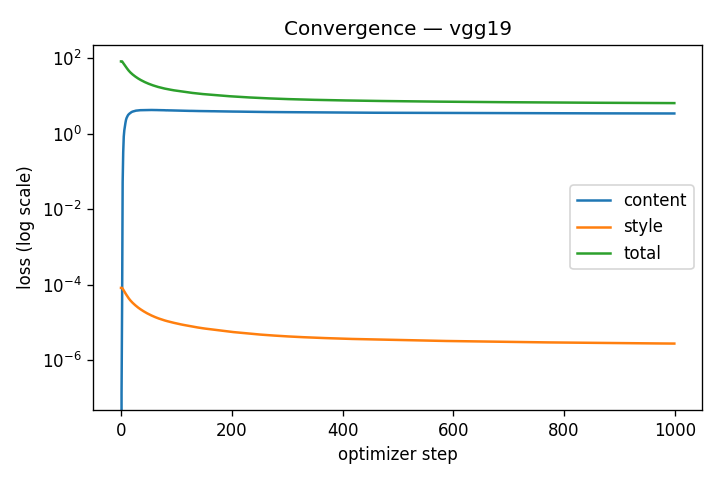
\includegraphics[width=0.49\textwidth]{loss_vgg19.png}
  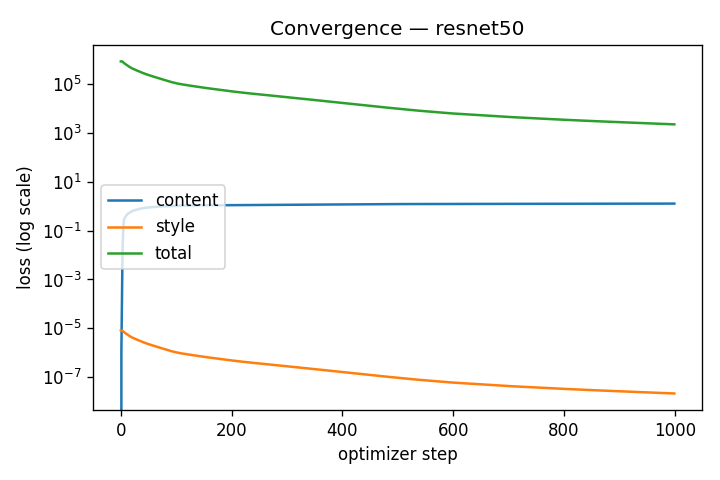
\includegraphics[width=0.49\textwidth]{loss_resnet50.png}
  \caption{Convergence curves (log scale) for VGG19 and ResNet50.}
  \label{fig:loss}
\end{figure}

\subsection{Additional content/style pairs}
To illustrate generality, the best backbone (VGG19) was applied to two further
pairs (Figs.~\ref{fig:mix2}--\ref{fig:mix3}): a still life rendered in the style
of Munch's \emph{The Scream}, and a photograph of an elephant rendered with a
high-contrast striped pattern.

\begin{figure}[ht]
  \centering
  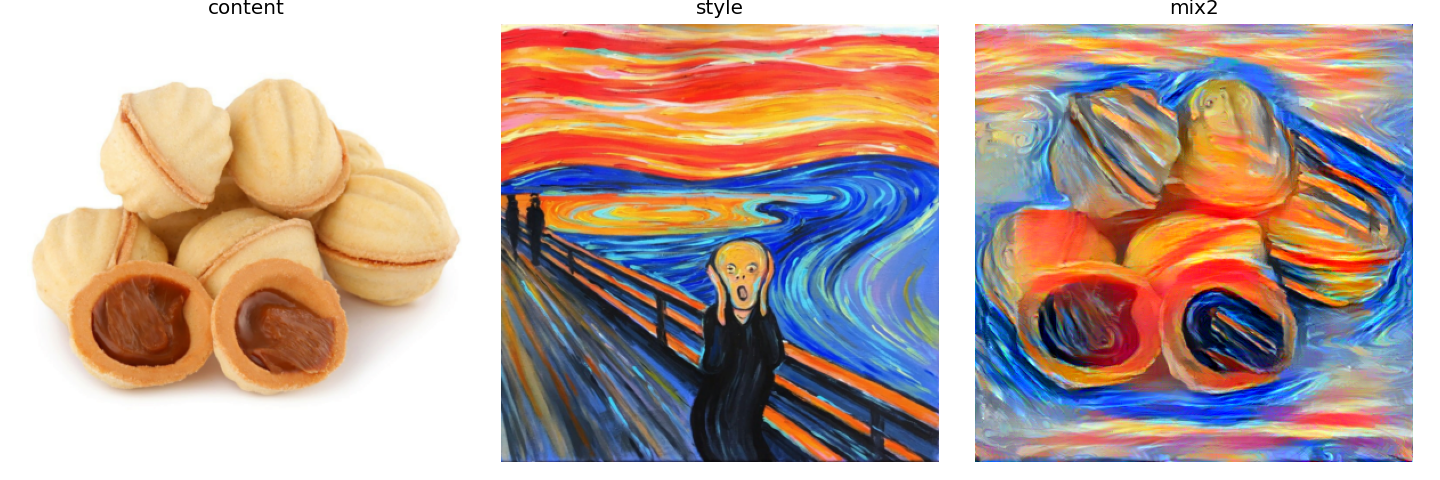
\includegraphics[width=0.8\textwidth]{triptych_mix2.png}
  \caption{Mix 2 --- content, style, result (VGG19).}
  \label{fig:mix2}
\end{figure}

\begin{figure}[ht]
  \centering
  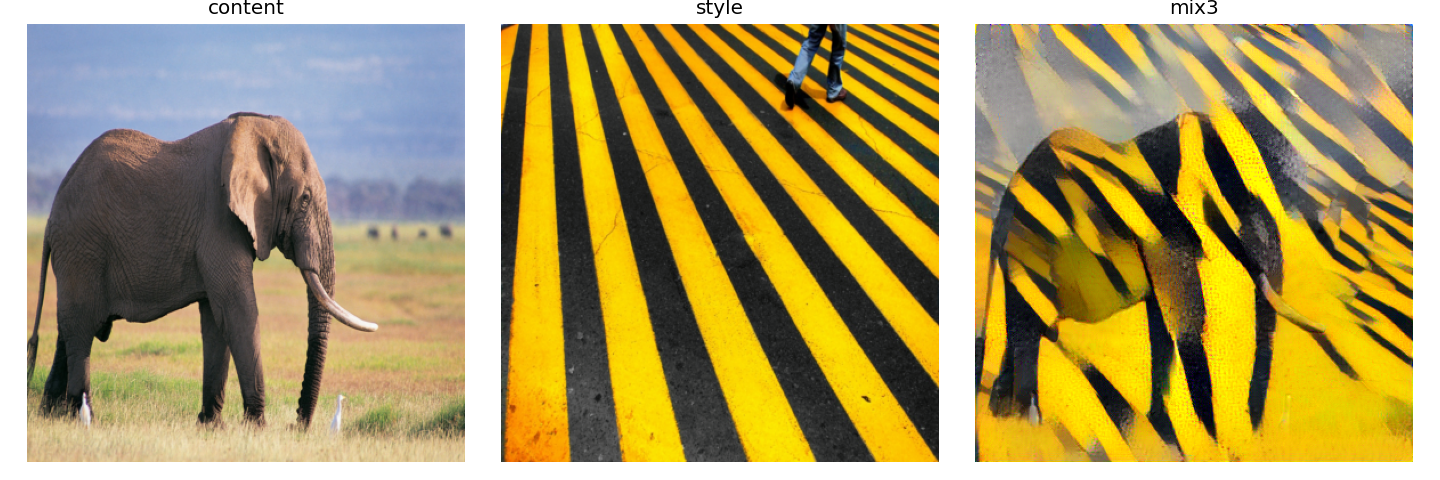
\includegraphics[width=0.8\textwidth]{triptych_mix3.png}
  \caption{Mix 3 --- content, style, result (VGG19).}
  \label{fig:mix3}
\end{figure}

\paragraph{Discussion.} ResNet50 consistently produces noisier results with
visible artifacts. A likely reason is that its residual connections and batch
normalization yield activations whose Gram statistics describe style texture
less faithfully than the sequential convolutional features of VGG. This explains
why VGG networks dominate the NST literature.

\section{Conclusion}
We implemented the classical style-transfer algorithm and compared three
feature-extractor architectures on the same image pair. VGG19 gave the best
stylization quality and ResNet50 the worst, and the method was demonstrated on
three different content/style pairs. These results agree with the common
practice of using VGG-family networks for neural style transfer.

\bibliographystyle{plain}
\bibliography{references}

\end{document}
